\chapter{Qualitätssicherung}
\label{chap:Qualitätssicherung}

Nach der erfolgreichen Implementierung des Übersetzers soll mit Hilfe einer zu testenden mobilen Anwendung überprüft werden,  ob der Compiler so arbeitet wie zu erwarten ist.  
\section{Testfälle}
Um den Compiler zu Testen ist es notwendig anhand vorher definierter Testfälle zu überprüfen, ob der Compiler die Xamarin.Forms App so übersetzt, wie es zu erwarten ist.   Zu diesem Zweck werden in diesem Abschnitt Testfälle definiert die sich aus den ermittelten Unterschieden zwischen beiden Frameworks,  sowie der Programmiersprachen ergeben. 

Tabelle \ref{tab:Testapp} zeigt die Testfälle für die Metadaten der mobilen Anwendung. 

\begin{table}[!ht]
\begin{tabularx}{\textwidth}{l|l|X}
   \textbf{ID} & \textbf{Komponente} & \textbf{Beschreibung} \\
\hline
1             & App-Icon           	& Prüfen ob das App-Icon übernommen wurde                      			 \\ 
2             & App-Name          	& Prüfen ob das App-Name übernommen wurde                      		 \\ 
3             & SDK Versionen      & Prüfen ob die SDK Versionen übernommen wurden                      \\ 
4             & Seitenname           				& In der Navigationsleiste wird der Name der aktuellen Seite angezeigt                      			 \\ 
5          	  & Navigation         			  	& Mit Hilfe des Menüs kann navigiert werden                      			 \\ 
6             & Zurück Navigation           	& Über die Navigationsleiste kann zurrück Navigiert werden                      			 \\ 
7             & Gyroscope auswerten           	& Die Werte werden in der App angezeigt.                      			 \\ 
8             & Accelerometer auswerten           	& Die Werte werden in der App angezeigt.                   			 \\ 
9            & Compass auswerten           	& Die Werte werden in der App angezeigt.                			 \\ 
10            & Magnetometer auswerten           	& Die Werte werden in der App angezeigt.                			 \\ 
11            & Sensor nicht verfügbar           	& Wenn ein Sensor nicht verfügbar ist, wird ein Fehler angezeigt          			 \\ 
12            & Steuerelemente wurden ausgetauscht           	& Alle Steuerelemente werden angezeigt        			 \\ 
13            & Ereignisse funktionieren           	&  Steuerelemente reagieren wie gewohnt     			 \\ 
14            & Bild aus Ressourcen laden           	& Ein Bild aus den Ressourcen wird in der App angezeigt                      			 \\ 
15             & Bild aus dem Web laden           	& Ein Bild aus dem Internet wird in der App                      			 \\ 
\end{tabularx}
\caption{Testfälle der Test App}
 \label{tab:Testapp}
\end{table}




\section{Testobjekt}
Anhand dieser Testfälle kann anschließend ein Xamarin.Forms Projekt erstellt werden, anhand welcher der Source-To-Source Compiler getestet werden kann.  Im folgenden werden die Funktionalitäten der mobilen Anwendung dargelegt und mit Hilfe von iOS Screenshots dargestellt,  die entsprechenden Android Screenshots werden der Vollständigkeitsannahme in \nameref{chap:AnhangAndroidScreenshots} dargestellt. 

Bei der Anwendung sind in einem ersten Schritt die Metadaten der Anwendung relevant.  Dazu gehören der Name der Anwendung sowie das Anwendungsicon - außerdem sollten die SDK Version der mobilen Anwendung nicht modifiziert werden. Nach dem Start der Anwendung wird eine Menustruktur angezeigt,  über den verschiedene Bereiche der Anwendung angesteuert werden können.  In Abbildung \ref{fig:TestObjectI} werden Screenshots der mobilen Anwendung gezeigt.

\begin{figure}[!ht]
 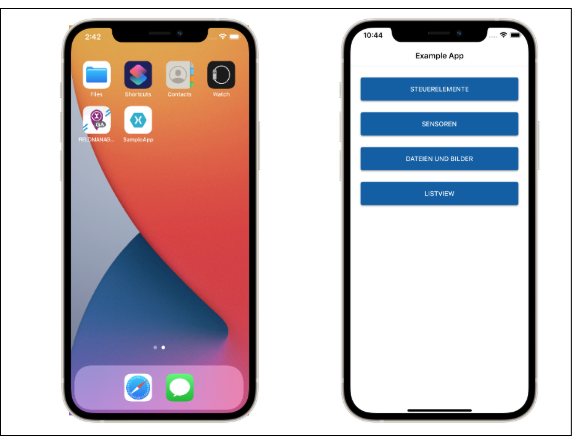
\includegraphics[width=\textwidth,keepaspectratio]{Images/Screenshot/AppIconAndMenu.png}
 \caption{Test Objekt Screenshots I}
 \label{fig:TestObjectI}
\end{figure}

Über dieses Menu kann der Anwender zu verschiedenen Seiten navigieren, die folgend kurz erläutert werden sollen.  Die in Abbildung \ref{fig:TestObjectII} zeigt die Seite mit den verfügbaren Steuerelementen von Xamarin.Forms,  wie sie auch in Kapitel 3 beschrieben wurden. Dazu gehören Ansichten für die Präsentation, für Interaktionen, zum setzen von Werten, für die Manipulation von Texten und für die Anzeige von aktuellen Interaktionen.
\begin{figure}[!ht]
 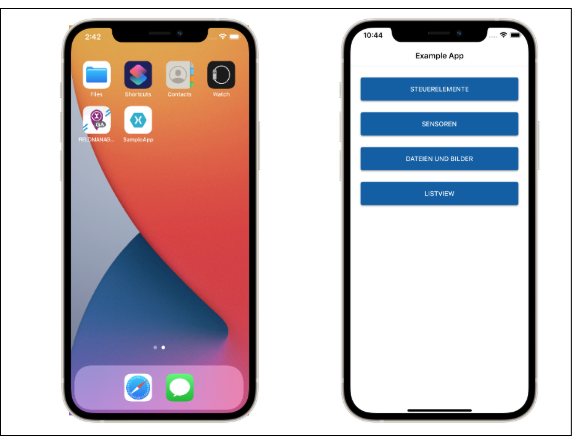
\includegraphics[width=\textwidth,keepaspectratio]{Images/Screenshot/AppIconAndMenu.png}
 \caption{Test Objekt Screenshots II}
 \label{fig:TestObjectII}
\end{figure}

Die folgende Option Sensoren öffnet eine Ansicht, auf der die aktuellen Werte von den Smartphone-Sensoren ausgegeben werden.  Diese Sensoren werden von vielen mobilen Anwendungen verwendet. Dazu gehören der Beschleunigungssensor, der Compass,  das Gyroscope und das Magnetometer.  Anhand dieser Seite,  soll sichergestellt werden, dass der Compiler auch die Funktionalität dieser Sensoren Abbilden kann. 

\begin{figure}[!ht]
 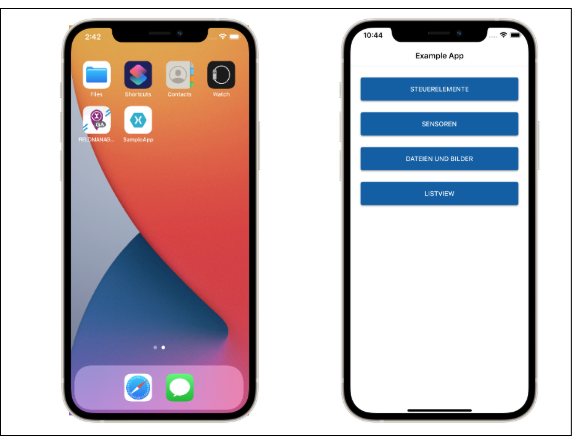
\includegraphics[width=\textwidth,keepaspectratio]{Images/Screenshot/AppIconAndMenu.png}
 \caption{Test Objekt Screenshots III}
 \label{fig:TestObjectIII}
\end{figure}

Ebenfalls werden in dem Testprojekt eine Liste und ein Carousel abgebildet,  da es sich bei diesen um häufig verwendete Elemente handelt - die in vielen mobilen Anwendungen verwendet wird. 

\begin{figure}[!ht]
 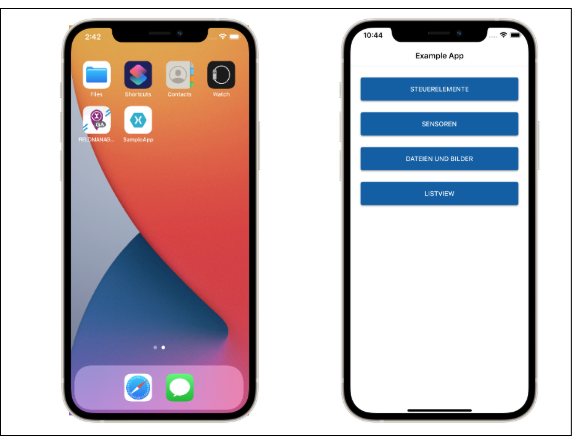
\includegraphics[width=\textwidth,keepaspectratio]{Images/Screenshot/AppIconAndMenu.png}
 \caption{Test Objekt Screenshots IV}
 \label{fig:TestObjectIV}
\end{figure}




\section{Testablauf}
Für den Start des Testlaufes wird die grafische Benutzeroberfläche gestartet. Anschließend wird das entwickelte Testobjekt als Xamarin.Forms Projekt und ein leerer als Ordner als Zielverzeichnis ausgewählt. Anschließend kann die Übersetzung gestartet werden.  Aufgrund der vielen Dateizugriffe und durchzuführenden Aktivitäten kann die Übersetzung der Anwendung eine gewisse Zeit in Anspruch nehmen. 
Nach dem erfolgreichen Durchlauf der Übersetzung werden im Front-End die Informationen bezüglich der Übersetzung ausgegeben.  
Anschließend kann mit Hilfe von Visual Studio Code die übersetzte Flutter Anwendung gestartet werden.  In einem ersten schritt können die Metadaten von sowohl Android als auch iOS App mit denen der Xamarin.Forms App verglichen werden, um zu validieren ob diese entsprechend übernommen wurden.
Nach einer erfolgreichen Überprüfung können nun die einzelnen Ansichten der Flutter App überprüft werden.  Dafür werden im folgenden die Screenshots der Flutter App dargestellt.  Dabei werden wie in der Einführung des Testobjektes die selben Bilder in der selben Reihenfolge dargestellt.  Die entsprechenden Screenshots von Android befinden sich ebenfalls im Anhang dieser Arbeit. 



\section{Testauswertung}

